\section*{Appendix A}

Results of experiments with the reward structures with different board sizes. 
\begin{figure}[h]
\centering
\makebox[\textwidth]{
	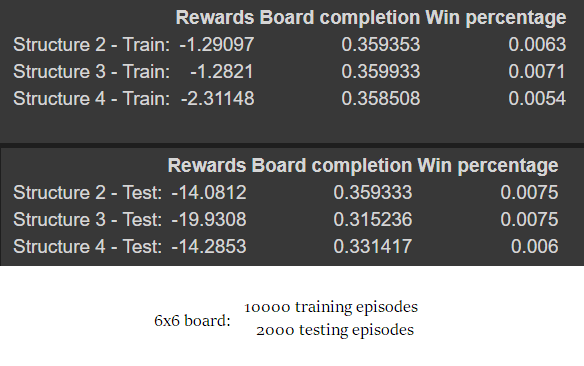
\includegraphics[width=0.55\textwidth]{reward-1.png}
	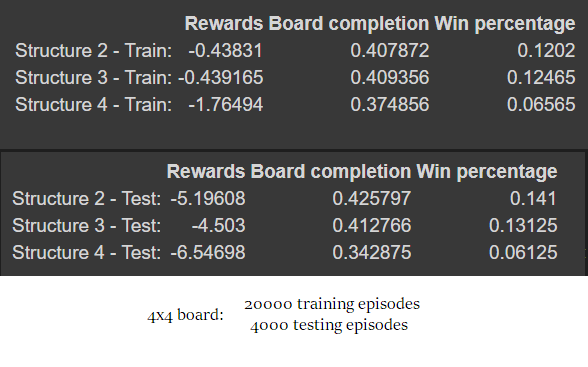
\includegraphics[width=0.55\textwidth]{reward-3.png}
}
\makebox[\textwidth]{
	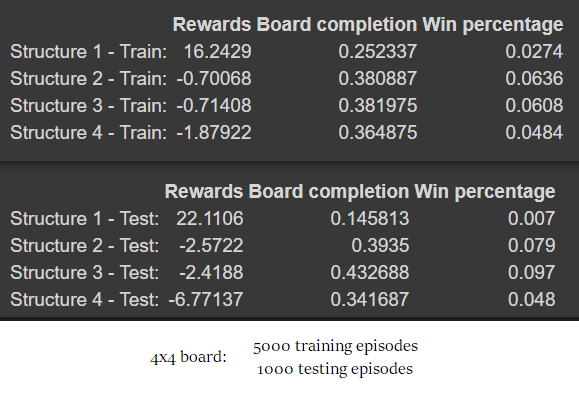
\includegraphics[width=0.55\textwidth]{reward-2.png}
	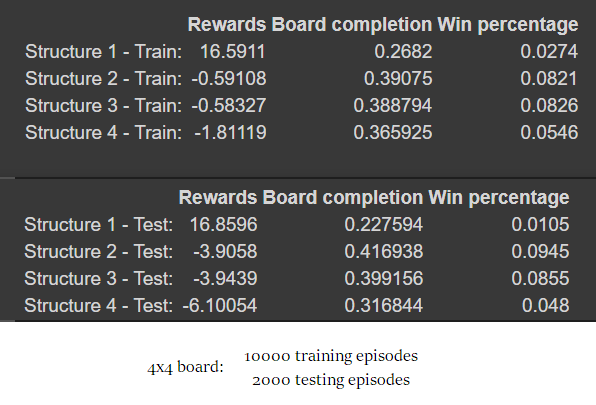
\includegraphics[width=0.55\textwidth]{reward-5.png}
}
\makebox[\textwidth]{
	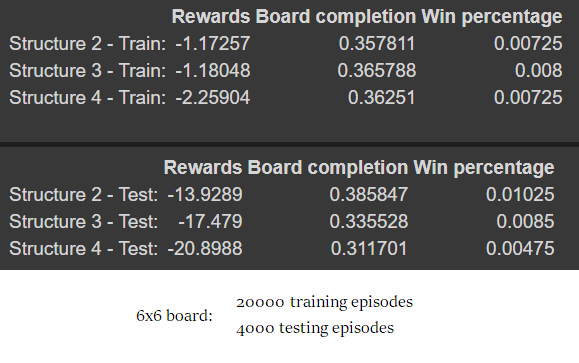
\includegraphics[width=0.55\textwidth]{reward-4.png}
}
\end{figure}

\newpage

\section*{Appendix B}

Score, win percentage, and board completion results from hyperparameter tuning.
\\\\
\textbf{Discount Rate}
\begin{figure}[h]
\centering
\makebox[\textwidth]{
	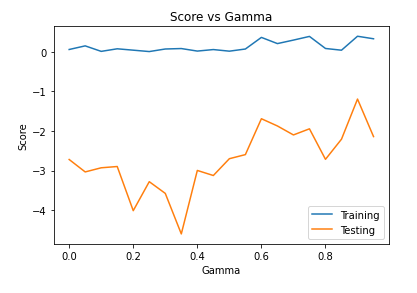
\includegraphics[width=0.4\textwidth]{gamma-score.png}
	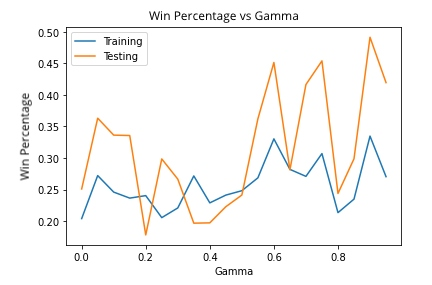
\includegraphics[width=0.4\textwidth]{gamma-win.jpg}
	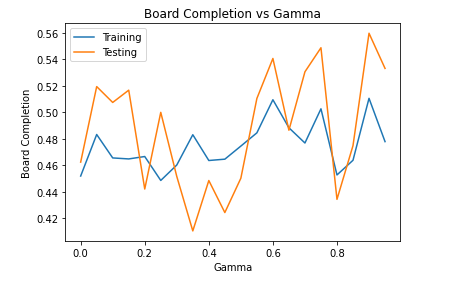
\includegraphics[width=0.4\textwidth]{gamma-board.png}
}
\end{figure}\\
\textbf{Learning Rate}
\begin{figure}[h]
\makebox[\textwidth]{
	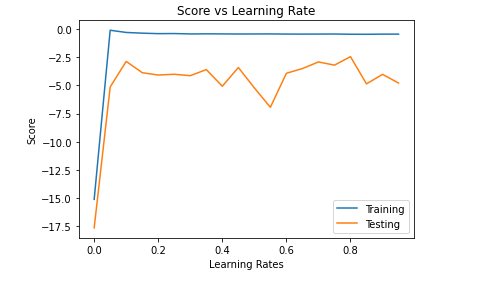
\includegraphics[width=0.4\textwidth]{alpha-score.png}
	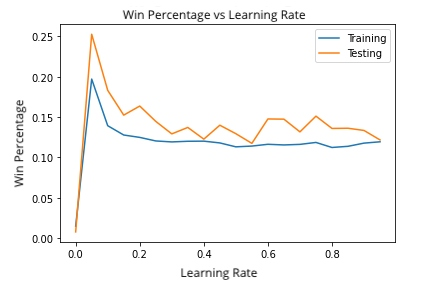
\includegraphics[width=0.4\textwidth]{alpha-win.jpg}
	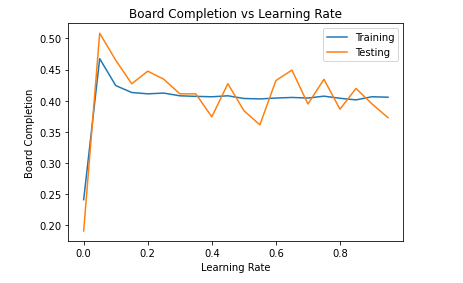
\includegraphics[width=0.4\textwidth]{alpha-board.png}
}
\end{figure}\\
\textbf{Minimum Exploration Rate}
\begin{figure}[h]
\makebox[\textwidth]{
	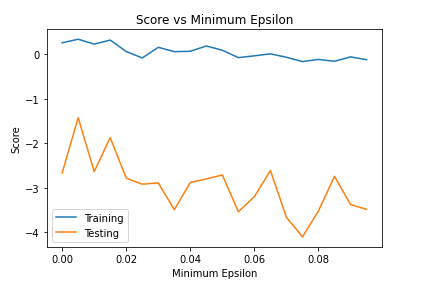
\includegraphics[width=0.4\textwidth]{epsilon-score.png}
	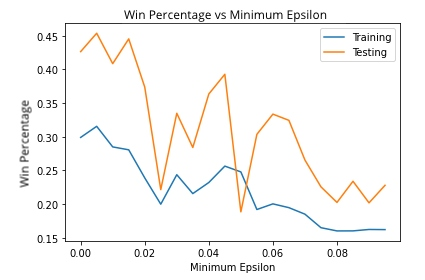
\includegraphics[width=0.4\textwidth]{epsilon-win.jpg}
	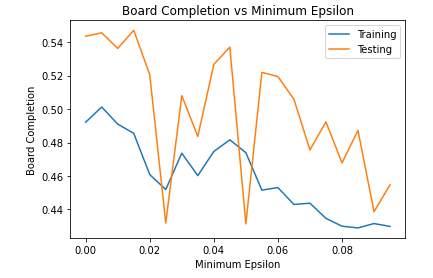
\includegraphics[width=0.4\textwidth]{epsilon-board.png}
}
\end{figure}
\newpage
\textbf{Exploration Decay Rate}
\begin{figure}[h]
\makebox[\textwidth]{
	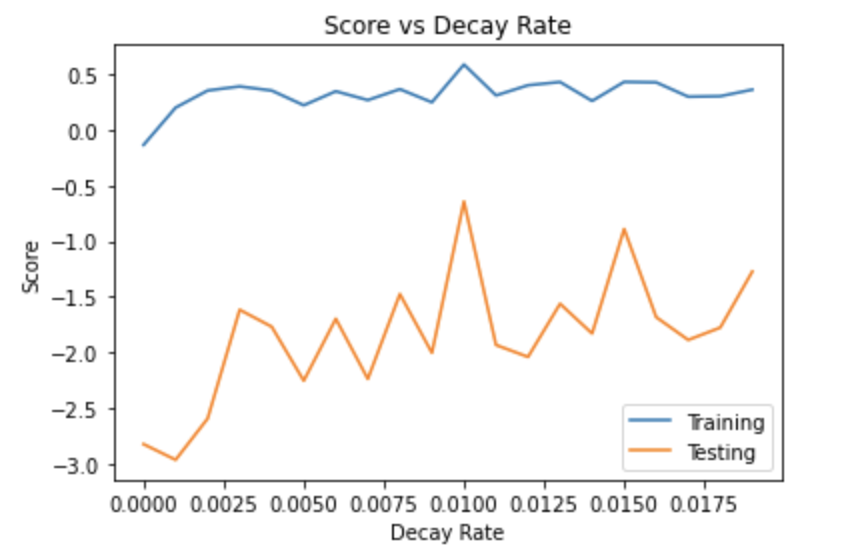
\includegraphics[width=0.4\textwidth]{decay-score.png}
	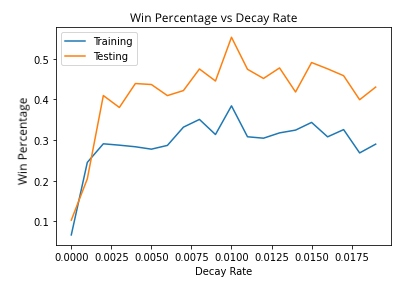
\includegraphics[width=0.4\textwidth]{decay-win.jpg}
	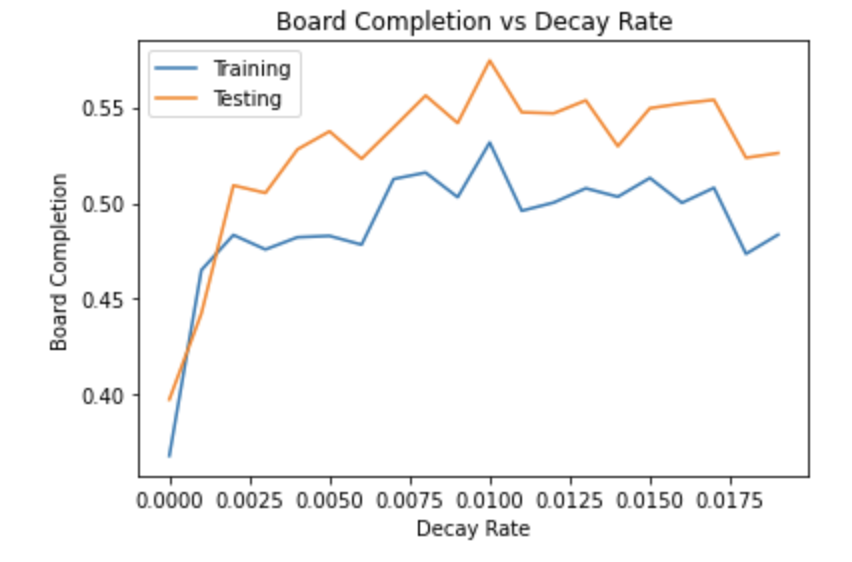
\includegraphics[width=0.4\textwidth]{decay-board.png}
}
\end{figure}

\newpage

\section*{Appendix C}

The 5-layer neural network used for the deep Q-learning agent.

\begin{figure}[h]
\centering
\makebox[\textwidth]{
	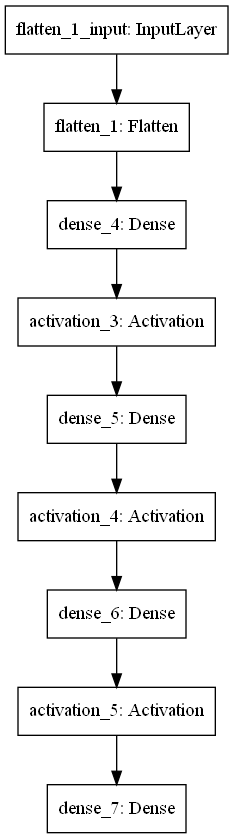
\includegraphics[width=0.3\textwidth]{dql-network.png}
}
\end{figure}